% Options for packages loaded elsewhere
% Options for packages loaded elsewhere
\PassOptionsToPackage{unicode}{hyperref}
\PassOptionsToPackage{hyphens}{url}
\PassOptionsToPackage{dvipsnames,svgnames,x11names}{xcolor}
%
\documentclass[
  letterpaper,
  DIV=11,
  numbers=noendperiod]{scrartcl}
\usepackage{xcolor}
\usepackage{amsmath,amssymb}
\setcounter{secnumdepth}{-\maxdimen} % remove section numbering
\usepackage{iftex}
\ifPDFTeX
  \usepackage[T1]{fontenc}
  \usepackage[utf8]{inputenc}
  \usepackage{textcomp} % provide euro and other symbols
\else % if luatex or xetex
  \usepackage{unicode-math} % this also loads fontspec
  \defaultfontfeatures{Scale=MatchLowercase}
  \defaultfontfeatures[\rmfamily]{Ligatures=TeX,Scale=1}
\fi
\usepackage{lmodern}
\ifPDFTeX\else
  % xetex/luatex font selection
\fi
% Use upquote if available, for straight quotes in verbatim environments
\IfFileExists{upquote.sty}{\usepackage{upquote}}{}
\IfFileExists{microtype.sty}{% use microtype if available
  \usepackage[]{microtype}
  \UseMicrotypeSet[protrusion]{basicmath} % disable protrusion for tt fonts
}{}
\makeatletter
\@ifundefined{KOMAClassName}{% if non-KOMA class
  \IfFileExists{parskip.sty}{%
    \usepackage{parskip}
  }{% else
    \setlength{\parindent}{0pt}
    \setlength{\parskip}{6pt plus 2pt minus 1pt}}
}{% if KOMA class
  \KOMAoptions{parskip=half}}
\makeatother
% Make \paragraph and \subparagraph free-standing
\makeatletter
\ifx\paragraph\undefined\else
  \let\oldparagraph\paragraph
  \renewcommand{\paragraph}{
    \@ifstar
      \xxxParagraphStar
      \xxxParagraphNoStar
  }
  \newcommand{\xxxParagraphStar}[1]{\oldparagraph*{#1}\mbox{}}
  \newcommand{\xxxParagraphNoStar}[1]{\oldparagraph{#1}\mbox{}}
\fi
\ifx\subparagraph\undefined\else
  \let\oldsubparagraph\subparagraph
  \renewcommand{\subparagraph}{
    \@ifstar
      \xxxSubParagraphStar
      \xxxSubParagraphNoStar
  }
  \newcommand{\xxxSubParagraphStar}[1]{\oldsubparagraph*{#1}\mbox{}}
  \newcommand{\xxxSubParagraphNoStar}[1]{\oldsubparagraph{#1}\mbox{}}
\fi
\makeatother

\usepackage{color}
\usepackage{fancyvrb}
\newcommand{\VerbBar}{|}
\newcommand{\VERB}{\Verb[commandchars=\\\{\}]}
\DefineVerbatimEnvironment{Highlighting}{Verbatim}{commandchars=\\\{\}}
% Add ',fontsize=\small' for more characters per line
\usepackage{framed}
\definecolor{shadecolor}{RGB}{241,243,245}
\newenvironment{Shaded}{\begin{snugshade}}{\end{snugshade}}
\newcommand{\AlertTok}[1]{\textcolor[rgb]{0.68,0.00,0.00}{#1}}
\newcommand{\AnnotationTok}[1]{\textcolor[rgb]{0.37,0.37,0.37}{#1}}
\newcommand{\AttributeTok}[1]{\textcolor[rgb]{0.40,0.45,0.13}{#1}}
\newcommand{\BaseNTok}[1]{\textcolor[rgb]{0.68,0.00,0.00}{#1}}
\newcommand{\BuiltInTok}[1]{\textcolor[rgb]{0.00,0.23,0.31}{#1}}
\newcommand{\CharTok}[1]{\textcolor[rgb]{0.13,0.47,0.30}{#1}}
\newcommand{\CommentTok}[1]{\textcolor[rgb]{0.37,0.37,0.37}{#1}}
\newcommand{\CommentVarTok}[1]{\textcolor[rgb]{0.37,0.37,0.37}{\textit{#1}}}
\newcommand{\ConstantTok}[1]{\textcolor[rgb]{0.56,0.35,0.01}{#1}}
\newcommand{\ControlFlowTok}[1]{\textcolor[rgb]{0.00,0.23,0.31}{\textbf{#1}}}
\newcommand{\DataTypeTok}[1]{\textcolor[rgb]{0.68,0.00,0.00}{#1}}
\newcommand{\DecValTok}[1]{\textcolor[rgb]{0.68,0.00,0.00}{#1}}
\newcommand{\DocumentationTok}[1]{\textcolor[rgb]{0.37,0.37,0.37}{\textit{#1}}}
\newcommand{\ErrorTok}[1]{\textcolor[rgb]{0.68,0.00,0.00}{#1}}
\newcommand{\ExtensionTok}[1]{\textcolor[rgb]{0.00,0.23,0.31}{#1}}
\newcommand{\FloatTok}[1]{\textcolor[rgb]{0.68,0.00,0.00}{#1}}
\newcommand{\FunctionTok}[1]{\textcolor[rgb]{0.28,0.35,0.67}{#1}}
\newcommand{\ImportTok}[1]{\textcolor[rgb]{0.00,0.46,0.62}{#1}}
\newcommand{\InformationTok}[1]{\textcolor[rgb]{0.37,0.37,0.37}{#1}}
\newcommand{\KeywordTok}[1]{\textcolor[rgb]{0.00,0.23,0.31}{\textbf{#1}}}
\newcommand{\NormalTok}[1]{\textcolor[rgb]{0.00,0.23,0.31}{#1}}
\newcommand{\OperatorTok}[1]{\textcolor[rgb]{0.37,0.37,0.37}{#1}}
\newcommand{\OtherTok}[1]{\textcolor[rgb]{0.00,0.23,0.31}{#1}}
\newcommand{\PreprocessorTok}[1]{\textcolor[rgb]{0.68,0.00,0.00}{#1}}
\newcommand{\RegionMarkerTok}[1]{\textcolor[rgb]{0.00,0.23,0.31}{#1}}
\newcommand{\SpecialCharTok}[1]{\textcolor[rgb]{0.37,0.37,0.37}{#1}}
\newcommand{\SpecialStringTok}[1]{\textcolor[rgb]{0.13,0.47,0.30}{#1}}
\newcommand{\StringTok}[1]{\textcolor[rgb]{0.13,0.47,0.30}{#1}}
\newcommand{\VariableTok}[1]{\textcolor[rgb]{0.07,0.07,0.07}{#1}}
\newcommand{\VerbatimStringTok}[1]{\textcolor[rgb]{0.13,0.47,0.30}{#1}}
\newcommand{\WarningTok}[1]{\textcolor[rgb]{0.37,0.37,0.37}{\textit{#1}}}

\usepackage{longtable,booktabs,array}
\usepackage{calc} % for calculating minipage widths
% Correct order of tables after \paragraph or \subparagraph
\usepackage{etoolbox}
\makeatletter
\patchcmd\longtable{\par}{\if@noskipsec\mbox{}\fi\par}{}{}
\makeatother
% Allow footnotes in longtable head/foot
\IfFileExists{footnotehyper.sty}{\usepackage{footnotehyper}}{\usepackage{footnote}}
\makesavenoteenv{longtable}
\usepackage{graphicx}
\makeatletter
\newsavebox\pandoc@box
\newcommand*\pandocbounded[1]{% scales image to fit in text height/width
  \sbox\pandoc@box{#1}%
  \Gscale@div\@tempa{\textheight}{\dimexpr\ht\pandoc@box+\dp\pandoc@box\relax}%
  \Gscale@div\@tempb{\linewidth}{\wd\pandoc@box}%
  \ifdim\@tempb\p@<\@tempa\p@\let\@tempa\@tempb\fi% select the smaller of both
  \ifdim\@tempa\p@<\p@\scalebox{\@tempa}{\usebox\pandoc@box}%
  \else\usebox{\pandoc@box}%
  \fi%
}
% Set default figure placement to htbp
\def\fps@figure{htbp}
\makeatother





\setlength{\emergencystretch}{3em} % prevent overfull lines

\providecommand{\tightlist}{%
  \setlength{\itemsep}{0pt}\setlength{\parskip}{0pt}}



 


\usepackage{booktabs}
\usepackage{longtable}
\usepackage{array}
\usepackage{multirow}
\usepackage{wrapfig}
\usepackage{float}
\usepackage{colortbl}
\usepackage{pdflscape}
\usepackage{tabu}
\usepackage{threeparttable}
\usepackage{threeparttablex}
\usepackage[normalem]{ulem}
\usepackage{makecell}
\usepackage{xcolor}
\KOMAoption{captions}{tableheading}
\makeatletter
\@ifpackageloaded{caption}{}{\usepackage{caption}}
\AtBeginDocument{%
\ifdefined\contentsname
  \renewcommand*\contentsname{Table of contents}
\else
  \newcommand\contentsname{Table of contents}
\fi
\ifdefined\listfigurename
  \renewcommand*\listfigurename{List of Figures}
\else
  \newcommand\listfigurename{List of Figures}
\fi
\ifdefined\listtablename
  \renewcommand*\listtablename{List of Tables}
\else
  \newcommand\listtablename{List of Tables}
\fi
\ifdefined\figurename
  \renewcommand*\figurename{Figure}
\else
  \newcommand\figurename{Figure}
\fi
\ifdefined\tablename
  \renewcommand*\tablename{Table}
\else
  \newcommand\tablename{Table}
\fi
}
\@ifpackageloaded{float}{}{\usepackage{float}}
\floatstyle{ruled}
\@ifundefined{c@chapter}{\newfloat{codelisting}{h}{lop}}{\newfloat{codelisting}{h}{lop}[chapter]}
\floatname{codelisting}{Listing}
\newcommand*\listoflistings{\listof{codelisting}{List of Listings}}
\makeatother
\makeatletter
\makeatother
\makeatletter
\@ifpackageloaded{caption}{}{\usepackage{caption}}
\@ifpackageloaded{subcaption}{}{\usepackage{subcaption}}
\makeatother
\usepackage{bookmark}
\IfFileExists{xurl.sty}{\usepackage{xurl}}{} % add URL line breaks if available
\urlstyle{same}
\hypersetup{
  pdftitle={2025年8月全国期货市场交易情况简报},
  pdfauthor={超级分析师Lixin Wu},
  colorlinks=true,
  linkcolor={blue},
  filecolor={Maroon},
  citecolor={Blue},
  urlcolor={Blue},
  pdfcreator={LaTeX via pandoc}}


\title{2025年8月全国期货市场交易情况简报}
\author{超级分析师Lixin Wu}
\date{2025-08-05}
\begin{document}
\maketitle


\section{中国期货市场月度分析报告}\label{ux4e2dux56fdux671fux8d27ux5e02ux573aux6708ux5ea6ux5206ux6790ux62a5ux544a}

\subsection{一、总体情况}\label{ux4e00ux603bux4f53ux60c5ux51b5}

\begin{Shaded}
\begin{Highlighting}[]
\CommentTok{\# 读取工作簿对象}
\NormalTok{wb }\OtherTok{\textless{}{-}} \FunctionTok{loadWorkbook}\NormalTok{(}\StringTok{"/Users/wulixin/Desktop/期货月报数据.xlsx"}\NormalTok{)}

\CommentTok{\# 获取特定工作表的数据}
\NormalTok{raw\_data }\OtherTok{\textless{}{-}} \FunctionTok{read.xlsx}\NormalTok{(wb, }\AttributeTok{sheet =}\StringTok{\textquotesingle{}7月\textquotesingle{}}\NormalTok{, }\AttributeTok{startRow =} \DecValTok{3}\NormalTok{, }\AttributeTok{colNames =} \ConstantTok{TRUE}\NormalTok{)}

\CommentTok{\# 这会为所有重复的列名添加后缀以使其唯一}
\NormalTok{new\_names }\OtherTok{\textless{}{-}} \FunctionTok{make.unique}\NormalTok{(}\FunctionTok{colnames}\NormalTok{(raw\_data), }\AttributeTok{sep =} \StringTok{"\_"}\NormalTok{)}
\FunctionTok{colnames}\NormalTok{(raw\_data) }\OtherTok{\textless{}{-}}\NormalTok{ new\_names}

\CommentTok{\# 步骤3: 现在可以安全地使用 fill()}
\NormalTok{cleaned\_data }\OtherTok{\textless{}{-}}\NormalTok{ raw\_data }\SpecialCharTok{\%\textgreater{}\%}
  \FunctionTok{fill}\NormalTok{(交易所名称, }\AttributeTok{.direction =} \StringTok{"down"}\NormalTok{) }\SpecialCharTok{\%\textgreater{}\%}
  \FunctionTok{filter}\NormalTok{(品种名称 }\SpecialCharTok{!=} \StringTok{"总计"}\NormalTok{)}

\CommentTok{\# 假设您的 clean\_data 已经存在,并且列名是您提供的那些(包含点号和下标)}
\CommentTok{\# 我们需要将这些列名修改为更规范、无歧义的名称}

\CommentTok{\# 使用 rename() 函数进行重命名}
\NormalTok{cleaned\_data }\OtherTok{\textless{}{-}}\NormalTok{ cleaned\_data }\SpecialCharTok{\%\textgreater{}\%}
  \CommentTok{\# 重新命名列,使用简洁、无特殊字符的名称}
  \FunctionTok{rename}\NormalTok{(}
    \AttributeTok{Exchange =} \StringTok{\textasciigrave{}}\AttributeTok{交易所名称}\StringTok{\textasciigrave{}}\NormalTok{,}
    \AttributeTok{Commodity =} \StringTok{\textasciigrave{}}\AttributeTok{品种名称}\StringTok{\textasciigrave{}}\NormalTok{,}
    \AttributeTok{Volume\_Jul =} \StringTok{\textasciigrave{}}\AttributeTok{本月成交量(手)}\StringTok{\textasciigrave{}}\NormalTok{,}
    \AttributeTok{Volume\_YoY =} \StringTok{\textasciigrave{}}\AttributeTok{去年同期成交量(手)}\StringTok{\textasciigrave{}}\NormalTok{,}
    \AttributeTok{Volume\_YoY\_Change =} \StringTok{\textasciigrave{}}\AttributeTok{同比增减(%)}\StringTok{\textasciigrave{}}\NormalTok{,}
    \AttributeTok{Volume\_Last\_Month =} \StringTok{\textasciigrave{}}\AttributeTok{上月成交量(手)}\StringTok{\textasciigrave{}}\NormalTok{,}
    \AttributeTok{Volume\_Ring\_Change =} \StringTok{\textasciigrave{}}\AttributeTok{环比增减(%)}\StringTok{\textasciigrave{}}\NormalTok{,}
    \AttributeTok{Volume\_Share\_National =} \StringTok{\textasciigrave{}}\AttributeTok{本月成交量占全国份额(%)}\StringTok{\textasciigrave{}}\NormalTok{,}
    \AttributeTok{Value\_Jul =} \StringTok{\textasciigrave{}}\AttributeTok{本月成交额.(亿元)}\StringTok{\textasciigrave{}}\NormalTok{, }
    \AttributeTok{Value\_YoY =} \StringTok{\textasciigrave{}}\AttributeTok{去年同期成交额(亿元)}\StringTok{\textasciigrave{}}\NormalTok{,}
    \AttributeTok{Value\_YoY\_Change =} \StringTok{\textasciigrave{}}\AttributeTok{同比增减(%)\_1}\StringTok{\textasciigrave{}}\NormalTok{,}
    \AttributeTok{Value\_Last\_Month =} \StringTok{\textasciigrave{}}\AttributeTok{上月成交额.(亿元)}\StringTok{\textasciigrave{}}\NormalTok{, }
    \AttributeTok{Value\_Ring\_Change =} \StringTok{\textasciigrave{}}\AttributeTok{环比增减(%)\_1}\StringTok{\textasciigrave{}}\NormalTok{,}
    \AttributeTok{Value\_Share\_National =} \StringTok{\textasciigrave{}}\AttributeTok{本月交易额占全国份额(%)}\StringTok{\textasciigrave{}}\NormalTok{,}
    \AttributeTok{Volume\_Cumulative =} \StringTok{\textasciigrave{}}\AttributeTok{今年累计成交总量(手)}\StringTok{\textasciigrave{}}\NormalTok{,}
    \AttributeTok{Volume\_Cumulative\_YoY =} \StringTok{\textasciigrave{}}\AttributeTok{去年同期成交总量(手)}\StringTok{\textasciigrave{}}\NormalTok{,}
    \AttributeTok{Volume\_Cumulative\_YoY\_Change =} \StringTok{\textasciigrave{}}\AttributeTok{同比增减(%)\_2}\StringTok{\textasciigrave{}}\NormalTok{,}
    \AttributeTok{Volume\_Cumulative\_Share =} \StringTok{\textasciigrave{}}\AttributeTok{今年累计成交总量占全国份额(\%)}\StringTok{\textasciigrave{}}\NormalTok{,}
    \AttributeTok{Value\_Cumulative =} \StringTok{\textasciigrave{}}\AttributeTok{今年累计成交总额(亿元)}\StringTok{\textasciigrave{}}\NormalTok{,}
    \AttributeTok{Value\_Cumulative\_YoY =} \StringTok{\textasciigrave{}}\AttributeTok{去年同期成交总额(亿元)}\StringTok{\textasciigrave{}}\NormalTok{,}
    \AttributeTok{Value\_Cumulative\_YoY\_Change =} \StringTok{\textasciigrave{}}\AttributeTok{同比增减(%)\_3}\StringTok{\textasciigrave{}}\NormalTok{,}
    \AttributeTok{Value\_Cumulative\_Share =} \StringTok{\textasciigrave{}}\AttributeTok{今年累计成交总额占全国份额(\%)}\StringTok{\textasciigrave{}}\NormalTok{,}
    \AttributeTok{Position\_End =} \StringTok{\textasciigrave{}}\AttributeTok{本月月末持仓量(手)}\StringTok{\textasciigrave{}}\NormalTok{,}
    \AttributeTok{Position\_Share\_National =} \StringTok{\textasciigrave{}}\AttributeTok{本月月末持仓量占全国份额(\%)}\StringTok{\textasciigrave{}}\NormalTok{,}
    \AttributeTok{Position\_Last\_Month =} \StringTok{\textasciigrave{}}\AttributeTok{上月月末持仓量(手)}\StringTok{\textasciigrave{}}\NormalTok{,}
    \AttributeTok{Position\_Ring\_Change =} \StringTok{\textasciigrave{}}\AttributeTok{环比增减(%)\_2}\StringTok{\textasciigrave{}}
\NormalTok{  ) }\SpecialCharTok{\%\textgreater{}\%}
  \FunctionTok{mutate\_at}\NormalTok{(}\FunctionTok{vars}\NormalTok{(}\FunctionTok{starts\_with}\NormalTok{(}\StringTok{"Volume"}\NormalTok{), }\FunctionTok{starts\_with}\NormalTok{(}\StringTok{"Value"}\NormalTok{), }\FunctionTok{starts\_with}\NormalTok{(}\StringTok{"Position"}\NormalTok{)), as.numeric) }\SpecialCharTok{\%\textgreater{}\%}
  \FunctionTok{mutate\_at}\NormalTok{(}\FunctionTok{vars}\NormalTok{(}\FunctionTok{ends\_with}\NormalTok{(}\StringTok{"\_Change"}\NormalTok{), }\FunctionTok{ends\_with}\NormalTok{(}\StringTok{"\_Share"}\NormalTok{)), }\SpecialCharTok{\textasciitilde{}}\NormalTok{ . }\SpecialCharTok{/} \DecValTok{100}\NormalTok{)}

\CommentTok{\# 假设 df 已经是经过 fill() 和 rename() 处理后的 cleaned\_data}
\NormalTok{df }\OtherTok{\textless{}{-}}\NormalTok{ cleaned\_data}

\CommentTok{\# 1. 计算全国市场的总体数据(8月)}
\CommentTok{\# 注意:这里计算的是8月数据,而非7月}
\NormalTok{total\_volume\_aug }\OtherTok{\textless{}{-}}\NormalTok{ df }\SpecialCharTok{\%\textgreater{}\%}
  \CommentTok{\# 过滤掉品种为"总计"的行,避免重复计算}
  \FunctionTok{filter}\NormalTok{(Commodity }\SpecialCharTok{!=} \StringTok{"总计"}\NormalTok{) }\SpecialCharTok{\%\textgreater{}\%}
  \FunctionTok{summarise}\NormalTok{(}\AttributeTok{total =} \FunctionTok{sum}\NormalTok{(Volume\_Jul, }\AttributeTok{na.rm =} \ConstantTok{TRUE}\NormalTok{)) }\SpecialCharTok{\%\textgreater{}\%}  \CommentTok{\# 使用 Volume\_Jul (本月成交量)}
  \FunctionTok{pull}\NormalTok{(total)}

\NormalTok{total\_value\_aug }\OtherTok{\textless{}{-}}\NormalTok{ df }\SpecialCharTok{\%\textgreater{}\%}
  \FunctionTok{filter}\NormalTok{(Commodity }\SpecialCharTok{!=} \StringTok{"总计"}\NormalTok{) }\SpecialCharTok{\%\textgreater{}\%}
  \FunctionTok{summarise}\NormalTok{(}\AttributeTok{total =} \FunctionTok{sum}\NormalTok{(Value\_Jul, }\AttributeTok{na.rm =} \ConstantTok{TRUE}\NormalTok{)) }\SpecialCharTok{\%\textgreater{}\%}   \CommentTok{\# 使用 Value\_Jul (本月成交额)}
  \FunctionTok{pull}\NormalTok{(total)}

\CommentTok{\# 2. 计算全国市场的累计数据(1{-}8月)}
\NormalTok{total\_volume\_1to8 }\OtherTok{\textless{}{-}}\NormalTok{ df }\SpecialCharTok{\%\textgreater{}\%}
  \FunctionTok{filter}\NormalTok{(Commodity }\SpecialCharTok{!=} \StringTok{"总计"}\NormalTok{) }\SpecialCharTok{\%\textgreater{}\%}
  \FunctionTok{summarise}\NormalTok{(}\AttributeTok{total =} \FunctionTok{sum}\NormalTok{(Volume\_Cumulative, }\AttributeTok{na.rm =} \ConstantTok{TRUE}\NormalTok{)) }\SpecialCharTok{\%\textgreater{}\%}  \CommentTok{\# 使用 Volume\_Cumulative}
  \FunctionTok{pull}\NormalTok{(total)}

\NormalTok{total\_value\_1to8 }\OtherTok{\textless{}{-}}\NormalTok{ df }\SpecialCharTok{\%\textgreater{}\%}
  \FunctionTok{filter}\NormalTok{(Commodity }\SpecialCharTok{!=} \StringTok{"总计"}\NormalTok{) }\SpecialCharTok{\%\textgreater{}\%}
  \FunctionTok{summarise}\NormalTok{(}\AttributeTok{total =} \FunctionTok{sum}\NormalTok{(Value\_Cumulative, }\AttributeTok{na.rm =} \ConstantTok{TRUE}\NormalTok{)) }\SpecialCharTok{\%\textgreater{}\%}   \CommentTok{\# 使用 Value\_Cumulative}
  \FunctionTok{pull}\NormalTok{(total)}

\CommentTok{\# 3. 获取同比增长率(直接从知识库或数据中提取)}
\CommentTok{\# 根据知识库内容,我们可以直接获取增长率,或者从数据中计算}
\CommentTok{\# 方法A: 直接引用知识库中的已知增长率 (推荐,因为数据更准确)}
\NormalTok{yoy\_vol\_jul\_percentage }\OtherTok{\textless{}{-}} \FloatTok{13.98} \CommentTok{\# 8月成交量同比增长率 (\%)}
\NormalTok{yoy\_val\_jul\_percentage }\OtherTok{\textless{}{-}} \FloatTok{21.38} \CommentTok{\# 8月成交额同比增长率 (\%)}

\NormalTok{yoy\_vol\_1to8\_percentage }\OtherTok{\textless{}{-}} \FloatTok{21.74} \CommentTok{\# 1{-}8月累计成交量同比增长率 (\%)}
\NormalTok{yoy\_val\_1to8\_percentage }\OtherTok{\textless{}{-}} \FloatTok{22.85} \CommentTok{\# 1{-}8月累计成交额同比增长率 (\%)}

\CommentTok{\# 方法B: 如果需要从数据中计算,可以这样:}
\CommentTok{\# yoy\_vol\_jul\_percentage \textless{}{-} (total\_volume\_aug {-} total\_volume\_yoy\_aug) / total\_volume\_yoy\_aug * 100}
\CommentTok{\# 但这需要您有 \textquotesingle{}去年同期成交量\textquotesingle{} 的全国总和,通常也需要对各交易所求和。}

\CommentTok{\# 4. 输出文字摘要 (基于知识库信息和计算结果)}
\FunctionTok{cat}\NormalTok{(}\StringTok{"根据中国期货业协会最新统计数据,以单边计算,2025年8月全国期货市场成交量为 "}\NormalTok{, }
    \FunctionTok{format}\NormalTok{(}\FunctionTok{round}\NormalTok{(total\_volume\_aug), }\AttributeTok{big.mark=}\StringTok{","}\NormalTok{), }\StringTok{"手,"}\NormalTok{, }
    \StringTok{"成交额为 "}\NormalTok{, }\FunctionTok{format}\NormalTok{(}\FunctionTok{round}\NormalTok{(total\_value\_aug), }\AttributeTok{big.mark=}\StringTok{","}\NormalTok{) , }\StringTok{"亿元,"}\NormalTok{,}
    \StringTok{"同比分别增长 "}\NormalTok{, yoy\_vol\_jul\_percentage, }\StringTok{"\% 和 "}\NormalTok{, yoy\_val\_jul\_percentage, }\StringTok{"\%。}\SpecialCharTok{\textbackslash{}n\textbackslash{}n}\StringTok{"}\NormalTok{)}
\end{Highlighting}
\end{Shaded}

\begin{verbatim}
根据中国期货业协会最新统计数据,以单边计算,2025年8月全国期货市场成交量为  1,058,719,289 手, 成交额为  713,124 亿元, 同比分别增长  13.98 % 和  21.38 %。
\end{verbatim}

\begin{Shaded}
\begin{Highlighting}[]
\FunctionTok{cat}\NormalTok{(}\StringTok{"1{-}8月全国期货市场累计成交量为 "}\NormalTok{, }
    \FunctionTok{format}\NormalTok{(}\FunctionTok{round}\NormalTok{(total\_volume\_1to8), }\AttributeTok{big.mark=}\StringTok{","}\NormalTok{), }\StringTok{"手,"}\NormalTok{,}
    \StringTok{"累计成交额为 "}\NormalTok{, }\FunctionTok{format}\NormalTok{(}\FunctionTok{round}\NormalTok{(total\_value\_1to8), }\AttributeTok{big.mark=}\StringTok{","}\NormalTok{) , }\StringTok{"亿元,"}\NormalTok{,}
    \StringTok{"同比分别增长 "}\NormalTok{, yoy\_vol\_1to8\_percentage, }\StringTok{"\% 和 "}\NormalTok{, yoy\_val\_1to8\_percentage, }\StringTok{"\%。}\SpecialCharTok{\textbackslash{}n}\StringTok{"}\NormalTok{)}
\end{Highlighting}
\end{Shaded}

\begin{verbatim}
1-8月全国期货市场累计成交量为  5,135,133,014 手, 累计成交额为  4,110,403 亿元, 同比分别增长  21.74 % 和  22.85 %。
\end{verbatim}

\subsection{二、交易所分析}\label{ux4e8cux4ea4ux6613ux6240ux5206ux6790}

\begin{Shaded}
\begin{Highlighting}[]
\CommentTok{\# 假设 df 已经是经过 fill() 和 rename() 处理后的 cleaned\_data}
\NormalTok{df }\OtherTok{\textless{}{-}}\NormalTok{ cleaned\_data}

\CommentTok{\# 提取各交易所的数据(过滤掉“总计”行,并按交易所分组求和)}
\NormalTok{exchange\_data }\OtherTok{\textless{}{-}}\NormalTok{ df }\SpecialCharTok{\%\textgreater{}\%}
  \CommentTok{\# 过滤掉 Commodity 为 "总计" 的行,避免重复计算}
  \FunctionTok{filter}\NormalTok{(Commodity }\SpecialCharTok{!=} \StringTok{"总计"}\NormalTok{) }\SpecialCharTok{\%\textgreater{}\%}
  \CommentTok{\# 按交易所分组}
  \FunctionTok{group\_by}\NormalTok{(Exchange) }\SpecialCharTok{\%\textgreater{}\%}
  \CommentTok{\# 计算每个交易所的总成交量、总成交额,并获取其市场份额和同比增长率}
  \FunctionTok{summarise}\NormalTok{(}
    \AttributeTok{Volume\_Aug =} \FunctionTok{sum}\NormalTok{(Volume\_Jul, }\AttributeTok{na.rm =} \ConstantTok{TRUE}\NormalTok{),           }\CommentTok{\# 本月成交量(手) {-}\textgreater{} 8月总成交量}
    \AttributeTok{Value\_Aug =} \FunctionTok{sum}\NormalTok{(Value\_Jul, }\AttributeTok{na.rm =} \ConstantTok{TRUE}\NormalTok{),             }\CommentTok{\# 本月成交额.(亿元) {-}\textgreater{} 8月总成交额}
    \AttributeTok{Share\_Volume =} \FunctionTok{first}\NormalTok{(Volume\_Share\_National),          }\CommentTok{\# 本月成交量占全国份额(%),取第一个非NA值}
    \AttributeTok{Share\_Value =} \FunctionTok{first}\NormalTok{(Value\_Share\_National),            }\CommentTok{\# 本月交易额占全国份额(%)}
    \AttributeTok{YoY\_Volume =} \FunctionTok{first}\NormalTok{(Volume\_YoY\_Change }\SpecialCharTok{*} \DecValTok{100}\NormalTok{),          }\CommentTok{\# 同比增减(%),注意:原始数据可能是小数,*100转为百分比}
    \AttributeTok{YoY\_Value =} \FunctionTok{first}\NormalTok{(Value\_YoY\_Change }\SpecialCharTok{*} \DecValTok{100}\NormalTok{)             }\CommentTok{\# 同比增减(%)\_1}
\NormalTok{  ) }\SpecialCharTok{\%\textgreater{}\%}
  \CommentTok{\# 取消分组}
  \FunctionTok{ungroup}\NormalTok{() }\SpecialCharTok{\%\textgreater{}\%}
  \CommentTok{\# 将市场份额和增长率从百分比形式转换为小数,便于后续处理}
  \FunctionTok{mutate}\NormalTok{(}
    \FunctionTok{across}\NormalTok{(}\FunctionTok{c}\NormalTok{(Share\_Volume, Share\_Value, YoY\_Volume, YoY\_Value), }\SpecialCharTok{\textasciitilde{}}\NormalTok{ . }\SpecialCharTok{/} \DecValTok{100}\NormalTok{)}
\NormalTok{  )}

\CommentTok{\# 创建一个更简洁的表格,只显示关键信息}
\NormalTok{exchange\_summary }\OtherTok{\textless{}{-}}\NormalTok{ exchange\_data }\SpecialCharTok{\%\textgreater{}\%}
  \FunctionTok{select}\NormalTok{(Exchange, Volume\_Aug, Value\_Aug, YoY\_Volume, YoY\_Value) }\SpecialCharTok{\%\textgreater{}\%}
  \CommentTok{\# 在生成表格时进行格式化,使其易于阅读}
  \FunctionTok{mutate}\NormalTok{(}
    \AttributeTok{Volume\_Aug =} \FunctionTok{format}\NormalTok{(}\FunctionTok{round}\NormalTok{(Volume\_Aug }\SpecialCharTok{/} \FloatTok{1e6}\NormalTok{, }\DecValTok{2}\NormalTok{), }\AttributeTok{big.mark=}\StringTok{","}\NormalTok{) }\SpecialCharTok{\%\textgreater{}\%} \FunctionTok{paste0}\NormalTok{(}\StringTok{"百万手"}\NormalTok{), }\CommentTok{\# 转换为百万手}
    \AttributeTok{Value\_Aug =} \FunctionTok{format}\NormalTok{(}\FunctionTok{round}\NormalTok{(Value\_Aug }\SpecialCharTok{/} \FloatTok{1e4}\NormalTok{, }\DecValTok{2}\NormalTok{), }\AttributeTok{big.mark=}\StringTok{","}\NormalTok{) }\SpecialCharTok{\%\textgreater{}\%} \FunctionTok{paste0}\NormalTok{(}\StringTok{"万亿元"}\NormalTok{),   }\CommentTok{\# 转换为万亿元}
    \AttributeTok{YoY\_Volume =} \FunctionTok{paste0}\NormalTok{(}\FunctionTok{round}\NormalTok{(YoY\_Volume }\SpecialCharTok{*} \DecValTok{100}\NormalTok{, }\DecValTok{2}\NormalTok{), }\StringTok{"\%"}\NormalTok{), }\CommentTok{\# 转换回百分比字符串}
    \AttributeTok{YoY\_Value =} \FunctionTok{paste0}\NormalTok{(}\FunctionTok{round}\NormalTok{(YoY\_Value }\SpecialCharTok{*} \DecValTok{100}\NormalTok{, }\DecValTok{2}\NormalTok{), }\StringTok{"\%"}\NormalTok{)}
\NormalTok{  )}

\CommentTok{\# 渲染表格}
\FunctionTok{kable}\NormalTok{(exchange\_summary, }\AttributeTok{caption =} \StringTok{"2025年8月各交易所交易情况"}\NormalTok{, }\AttributeTok{booktabs =} \ConstantTok{TRUE}\NormalTok{, }\AttributeTok{escape =} \ConstantTok{FALSE}\NormalTok{) }\SpecialCharTok{\%\textgreater{}\%}
  \FunctionTok{kable\_styling}\NormalTok{(}\AttributeTok{font\_size =} \DecValTok{10}\NormalTok{, }\AttributeTok{full\_width =} \ConstantTok{TRUE}\NormalTok{) }\SpecialCharTok{\%\textgreater{}\%}
  \FunctionTok{add\_header\_above}\NormalTok{(}\FunctionTok{c}\NormalTok{(}\StringTok{" "} \OtherTok{=} \DecValTok{1}\NormalTok{, }\StringTok{"8月"} \OtherTok{=} \DecValTok{2}\NormalTok{, }\StringTok{"同比增长"} \OtherTok{=} \DecValTok{2}\NormalTok{))}
\end{Highlighting}
\end{Shaded}

\begin{table}

\caption{\label{tab:unnamed-chunk-2}2025年8月各交易所交易情况}
\centering
\fontsize{10}{12}\selectfont
\begin{tabu} to \linewidth {>{\raggedright}X>{\raggedright}X>{\raggedright}X>{\raggedright}X>{\raggedright}X}
\toprule
\multicolumn{1}{c}{ } & \multicolumn{2}{c}{8月} & \multicolumn{2}{c}{同比增长} \\
\cmidrule(l{3pt}r{3pt}){2-3} \cmidrule(l{3pt}r{3pt}){4-5}
Exchange & Volume_Aug & Value_Aug & YoY_Volume & YoY_Value\\
\midrule
上海国际能源交易中心 & 14.61百万手 & 2.78万亿元 & 0.35% & 0.14%\\
上海期货交易所 & 229.14百万手 & 19.57万亿元 & -0.24% & -0.22%\\
中国金融期货交易所 & 25.16百万手 & 20.64万亿元 & 0.22% & 0.43%\\
大连商品交易所 & 273.68百万手 & 11.46万亿元 & 0.59% & 0.44%\\
广州期货交易所 & 115.15百万手 & 6.54万亿元 & 2.02% & 1.41%\\
\addlinespace
郑州商品交易所 & 400.98百万手 & 10.33万亿元 & -0.19% & -0.22%\\
\bottomrule
\end{tabu}
\end{table}

\begin{Shaded}
\begin{Highlighting}[]
\CommentTok{\# 绘制成交量柱状图}
\CommentTok{\# 注意:这里需要使用未格式化的原始数值 (Volume\_Aug),而不是已经变成字符的 "百万手"}
\FunctionTok{ggplot}\NormalTok{(exchange\_data, }\FunctionTok{aes}\NormalTok{(}\AttributeTok{x =} \FunctionTok{reorder}\NormalTok{(Exchange, Volume\_Aug), }\AttributeTok{y =}\NormalTok{ Volume\_Aug, }\AttributeTok{fill =}\NormalTok{ Exchange)) }\SpecialCharTok{+}
  \FunctionTok{geom\_col}\NormalTok{() }\SpecialCharTok{+}
  \FunctionTok{coord\_flip}\NormalTok{() }\SpecialCharTok{+}
  \FunctionTok{theme\_minimal}\NormalTok{() }\SpecialCharTok{+}
  \FunctionTok{scale\_y\_continuous}\NormalTok{(}\AttributeTok{labels =} \ControlFlowTok{function}\NormalTok{(x) }\FunctionTok{format}\NormalTok{(x }\SpecialCharTok{/} \FloatTok{1e6}\NormalTok{, }\AttributeTok{big.mark =} \StringTok{","}\NormalTok{)) }\SpecialCharTok{+} \CommentTok{\# Y轴标签显示为"百万手"}
  \FunctionTok{labs}\NormalTok{(}\AttributeTok{title =} \StringTok{"2025年8月各交易所成交量"}\NormalTok{,}
       \AttributeTok{x =} \StringTok{""}\NormalTok{, }
       \AttributeTok{y =} \StringTok{"成交量 (百万手)"}\NormalTok{) }\SpecialCharTok{+}
  \FunctionTok{theme}\NormalTok{(}\AttributeTok{legend.position =} \StringTok{"none"}\NormalTok{)}
\end{Highlighting}
\end{Shaded}

\pandocbounded{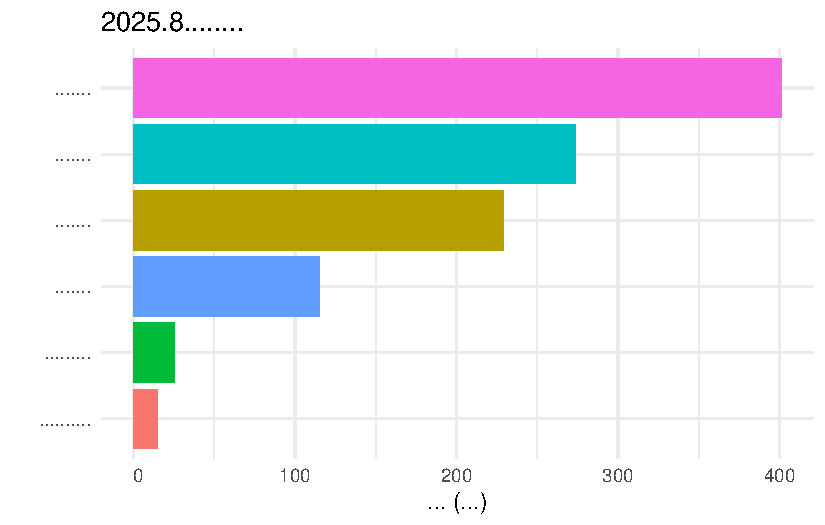
\includegraphics[keepaspectratio]{测试pdf_files/figure-pdf/unnamed-chunk-3-1.pdf}}

\begin{Shaded}
\begin{Highlighting}[]
\CommentTok{\# 绘制成交额柱状图}
\FunctionTok{ggplot}\NormalTok{(exchange\_data, }\FunctionTok{aes}\NormalTok{(}\AttributeTok{x =} \FunctionTok{reorder}\NormalTok{(Exchange, Value\_Aug), }\AttributeTok{y =}\NormalTok{ Value\_Aug, }\AttributeTok{fill =}\NormalTok{ Exchange)) }\SpecialCharTok{+}
  \FunctionTok{geom\_col}\NormalTok{() }\SpecialCharTok{+}
  \FunctionTok{coord\_flip}\NormalTok{() }\SpecialCharTok{+}
  \FunctionTok{theme\_minimal}\NormalTok{() }\SpecialCharTok{+}
  \FunctionTok{scale\_y\_continuous}\NormalTok{(}\AttributeTok{labels =} \ControlFlowTok{function}\NormalTok{(x) }\FunctionTok{format}\NormalTok{(x }\SpecialCharTok{/} \FloatTok{1e4}\NormalTok{, }\AttributeTok{big.mark =} \StringTok{","}\NormalTok{)) }\SpecialCharTok{+} \CommentTok{\# Y轴标签显示为"万亿元"}
  \FunctionTok{labs}\NormalTok{(}\AttributeTok{title =} \StringTok{"2025年8月各交易所成交额"}\NormalTok{,}
       \AttributeTok{x =} \StringTok{""}\NormalTok{, }
       \AttributeTok{y =} \StringTok{"成交额 (万亿元)"}\NormalTok{) }\SpecialCharTok{+}
  \FunctionTok{theme}\NormalTok{(}\AttributeTok{legend.position =} \StringTok{"none"}\NormalTok{)}
\end{Highlighting}
\end{Shaded}

\pandocbounded{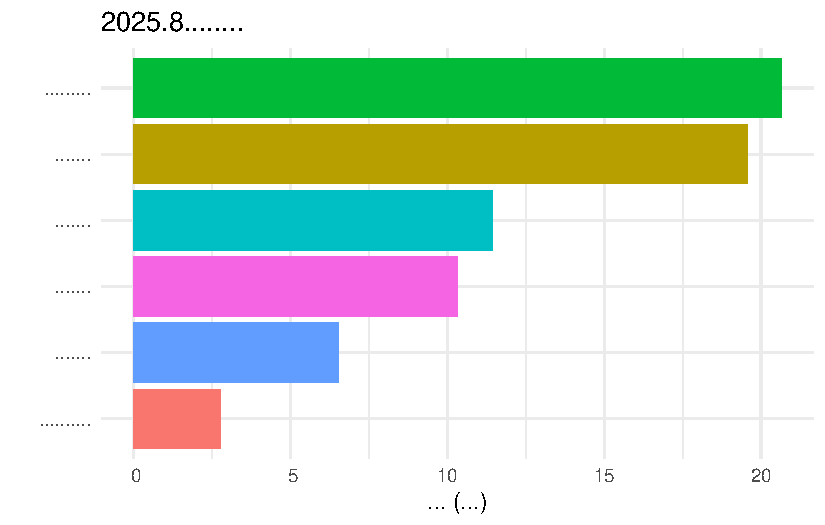
\includegraphics[keepaspectratio]{测试pdf_files/figure-pdf/unnamed-chunk-4-1.pdf}}




\end{document}
